\documentclass[french, a4paper, 12pt]{article}
\newcommand{\docname}{Les révolutionnaires boisais}
% Layout
\usepackage{fancyhdr, fancyvrb}
\usepackage{lastpage}
\usepackage[left=2.0cm, right=2.0cm, top = 2.0cm, bottom = 2.0cm]{geometry}
\usepackage{multicol}
\usepackage{graphicx}
\usepackage{hyperref}
\hypersetup{hyperindex=true, colorlinks, linkcolor=blue, urlcolor=blue, citecolor=blue, breaklinks=true}
\everymath{\displaystyle}


% Language
\usepackage[utf8]{inputenc}
\usepackage[T1]{fontenc}
\usepackage{babel}


% Pagestyle
\pagestyle{fancy}

\renewcommand{\headrulewidth}{0.4pt}
\renewcommand{\footrulewidth}{0.4pt}

\title{\sc \docname}
\date{}

\lhead{}
\rhead{\docname}
\cfoot{\thepage\ $|$ \pageref{LastPage}}
\rfoot{Odyssée}

\begin{document} \maketitle \vspace{3pt} \hrule \vspace{3pt}

\tableofcontents

\section{Contexte}

En l'an 285, le Grand Duc de Boisia, Zayrïm, est assassiné par le peuple. Avec le soutient logistique et matériel du Royaume de Seresia, le peuple prend la tête du pays et pourchasse les anciens puissants. Mais il s'avère que les intérêts de Seresia et ceux du Grand Duché divergent. Le Royaume de Seresia affaibli de plus en plus le Grand Duché jusqu'à pouvoir l'annexer sans que ce dernier puisse opposer de résistance. Le peuple boisais en est bien conscient, mais ne peut pas montrer son mécontentement, le soutient financier de Seresia étant vital pour Boisia.

Cependant, dans l'ombre, le peuple s'organise, seul cette fois-ci, pour reprendre vraiment le contrôle de leur pays. Dans la ville de Solle, au sud est du pays, Frolorn mène une troupe de volontaires vers l'indépendance.

\section{Présentation du lieu}

\begin{figure}[htp]
\centering
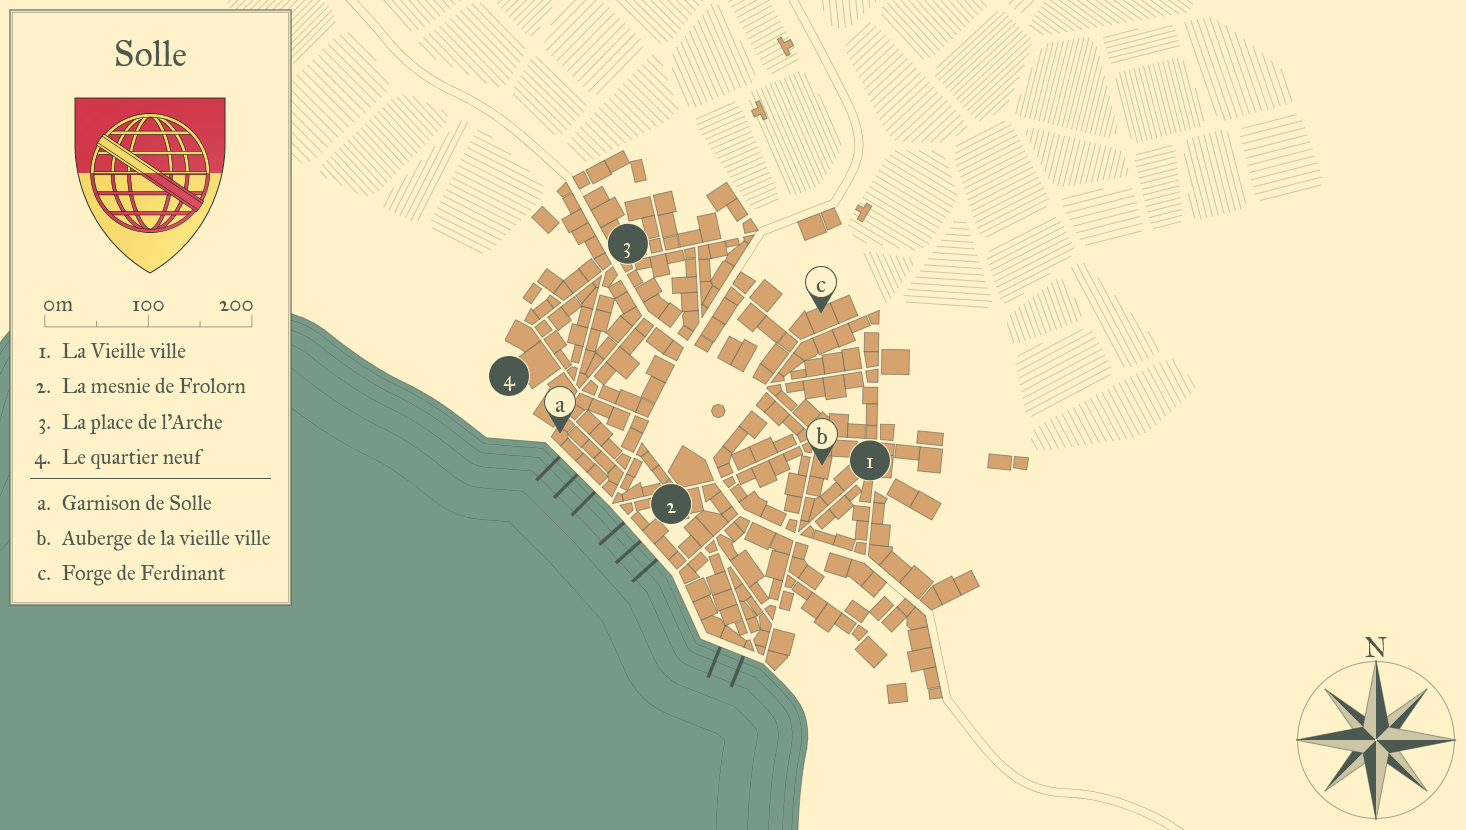
\includegraphics[width=18cm]{Cartes/Solle.png}
\caption{Solle}
\label{solle}
\end{figure}

Boisia est situé à l'extrémité est du pays, très boisé, le Grand Duché est difficile d'accès à une armée régulière et le terrain se prête plus à la mise en place de guet-apens qu'à la progression lourde et lente d'une armée complète.

La ferme de Frolorn sert de gîte à tous les révolutionnaires. Placé près du port où Forlorn a beaucoup de contact, la ville offre une possibilité de replis et les différents bâtiments de la mesnie communiquent par les caves. (voir Figure~\ref{solle})

\section{Intrigue}

La fureur de la révolution précédente se calme à peine que la prochaine gronde déjà. À Solle, le climat est tendu et frénétique. Les révolutionnaires ont pour l'instant fait quelques faits d'armes violents~: pillage d'entrepôts, enlèvement et demande de rançon, interseption des messagers… Mais depuis quelques temps, les échecs se multiplient pour le groupe… La présence d'une taupe n'est plus à démontrer.

\section{Quête principale}

\subsection{Arrivée à Boisia}

Déjà reconnu pour ses compétences en théologie, Narcisse le Grand a reçu le titre de Diplomate Officiel d'Otlin. Cette charge, aussi prestigieuse qu'exigente pour qui la détient, est en effet un gage de fidélité au gouvernement otlinois. Autrement dit, les Diplomates Officiels Otlinois sont tenus d'être au service de l'Empire.

Avec les récents évènements à Boisia, Otlin aimerait profiter de pactes commerciaux avec le nouveau gouvernement, les tentatives de contacts avec l'ex-Grand Duc n'ayant jamais été fructueuses. Mais l'instabilité du gouvernement post-révolutionnaire rend les alliances incertaines et l'ingérence de Seresia pourrait mettre en péril les relations naissantes entre Otlin et Boisia.

Le gouvernement d'Otlin attend donc que Seresia soit définitivement écarté de Boisia pour entamer de véritables tractations. Et c'est pour ça qu'il vous envoie.

\subsection{Quête}

Vous devez aider les révolutionnaires et favoriser l'expulsion des seresiens du gouvernement boisais. Pour cela, vous devrez identifier et éliminer la taupe. Toutefois, si Seresia apprends votre présence en territoire boisais, les relations entre Otlin et Seresia vont devenir tendue ce qui n'est pas souhaitable. De plus, la précédente révolution ayant été une humiliation cuisante pour le peuple boisais à cause de l'ingérence seresienne, vous annoncer comme étant des étrangers au Grand Duché serait contreproductif.


\end{document}